\documentclass[aspectratio=169,10pt]{beamer}

\usepackage{iftex}
\providecommand{\dunenoirsetupfonts}{}
\newcommand{\DuneNoirLocalFontPath}{fonts}

\newcommand{\DuneNoirMonoFallback}{%
  \IfFontExistsTF{JetBrainsMono Nerd Font Propo}{
    \setmonofont{JetBrainsMono Nerd Font Propo}[Scale=0.92]
  }{
    \IfFontExistsTF{JetBrainsMono Nerd Font}{
      \setmonofont{JetBrainsMono Nerd Font}[Scale=0.92]
    }{
      \setmonofont{Courier New}[Scale=0.92]
    }
  }
}

\newcommand{\DuneNoirSansFallback}{%
  \IfFontExistsTF{IBM Plex Sans}{
    \setsansfont{IBM Plex Sans}
    \setmainfont{IBM Plex Sans}
  }{
    \IfFontExistsTF{Helvetica Neue}{
      \setsansfont{Helvetica Neue}
      \setmainfont{Helvetica Neue}
    }{
      \setsansfont{Arial}
      \setmainfont{Arial}
    }
  }
}

\newcommand{\DuneNoirUseHelvetica}{%
  \renewcommand{\dunenoirsetupfonts}{%
    \IfFontExistsTF{Helvetica Neue}{
      \setsansfont{Helvetica Neue}
      \setmainfont{Helvetica Neue}
    }{
      \IfFontExistsTF{Helvetica}{
        \setsansfont{Helvetica}
        \setmainfont{Helvetica}
      }{
        \DuneNoirSansFallback
      }
    }
    \DuneNoirMonoFallback
  }%
}

\newcommand{\DuneNoirUseOpenSans}{%
  \renewcommand{\dunenoirsetupfonts}{%
    \IfFileExists{\DuneNoirLocalFontPath/OpenSans.ttf}{
      \setsansfont{Open Sans Custom}[
        Path=\DuneNoirLocalFontPath/,
        UprightFont={OpenSans.ttf},
        ItalicFont={OpenSans-Italic.ttf},
        BoldFont={OpenSans.ttf},
        BoldItalicFont={OpenSans-Italic.ttf},
        BoldFeatures={FakeBold=1.45},
        BoldItalicFeatures={FakeBold=1.45}
      ]
      \setmainfont{Open Sans Custom}[
        Path=\DuneNoirLocalFontPath/,
        UprightFont={OpenSans.ttf},
        ItalicFont={OpenSans-Italic.ttf},
        BoldFont={OpenSans.ttf},
        BoldItalicFont={OpenSans-Italic.ttf},
        BoldFeatures={FakeBold=1.45},
        BoldItalicFeatures={FakeBold=1.45}
      ]
    }{
      \DuneNoirSansFallback
    }
    \DuneNoirMonoFallback
  }%
}

\newcommand{\DuneNoirUseDosis}{%
  \renewcommand{\dunenoirsetupfonts}{%
    \IfFileExists{\DuneNoirLocalFontPath/Dosis.ttf}{
      \setsansfont{Dosis Custom}[
        Path=\DuneNoirLocalFontPath/,
        UprightFont={Dosis.ttf},
        ItalicFont={Dosis.ttf},
        BoldFont={Dosis.ttf},
        BoldItalicFont={Dosis.ttf},
        ItalicFeatures={FakeSlant=0.16},
        BoldFeatures={FakeBold=1.6},
        BoldItalicFeatures={FakeBold=1.6,FakeSlant=0.16}
      ]
      \setmainfont{Dosis Custom}[
        Path=\DuneNoirLocalFontPath/,
        UprightFont={Dosis.ttf},
        ItalicFont={Dosis.ttf},
        BoldFont={Dosis.ttf},
        BoldItalicFont={Dosis.ttf},
        ItalicFeatures={FakeSlant=0.16},
        BoldFeatures={FakeBold=1.6},
        BoldItalicFeatures={FakeBold=1.6,FakeSlant=0.16}
      ]
    }{
      \DuneNoirSansFallback
    }
    \DuneNoirMonoFallback
  }%
}

\newcommand{\DuneNoirUseKoHo}{%
  \renewcommand{\dunenoirsetupfonts}{%
    \IfFileExists{\DuneNoirLocalFontPath/KoHo-Regular.ttf}{
      \setsansfont{KoHo Custom}[
        Path=\DuneNoirLocalFontPath/,
        UprightFont={KoHo-Regular.ttf},
        BoldFont={KoHo-Bold.ttf},
        ItalicFont={KoHo-Italic.ttf},
        BoldItalicFont={KoHo-BoldItalic.ttf}
      ]
      \setmainfont{KoHo Custom}[
        Path=\DuneNoirLocalFontPath/,
        UprightFont={KoHo-Regular.ttf},
        BoldFont={KoHo-Bold.ttf},
        ItalicFont={KoHo-Italic.ttf},
        BoldItalicFont={KoHo-BoldItalic.ttf}
      ]
    }{
      \DuneNoirSansFallback
    }
    \DuneNoirMonoFallback
  }%
}

\DuneNoirUseHelvetica
\makeatletter
\input{../dune_dark_template_lab/beamerthemeDUNENoir.sty}
\makeatother

\ifPDFTeX
  \usepackage[T1]{fontenc}
  \usepackage[utf8]{inputenc}
\fi

\usepackage{amsmath,amssymb}
\usepackage{array,booktabs,tabularx}
\usepackage{graphicx}
\usepackage{hyperref}
\usepackage{siunitx}
\usepackage{tikz}
\usetikzlibrary{arrows.meta,calc,positioning,fit,shapes.geometric,decorations.pathreplacing}

\title[DAPHNE PRR Readiness]{DAPHNE Production Readiness Review}
\subtitle{A reviewer-facing map of evidence, risks, decisions, and fallbacks}
\author{Manuel Arroyave}
\date{Draft, May 2026}
\newcommand{\mydate}{Draft, May 2026}

\definecolor{okgreen}{HTML}{8FD6A9}
\definecolor{warnyellow}{HTML}{E7C547}
\definecolor{riskred}{HTML}{F28B82}
\definecolor{softblue}{HTML}{9BDCF2}
\definecolor{deepnavy}{HTML}{0D141C}

\newcommand{\eyebrow}[1]{{\color{noircyan}\small\bfseries #1\par}}
\newcommand{\tinycite}[1]{{\color{noirmuted}\tiny Source: #1\par}}
\newcommand{\oktag}{\textcolor{okgreen}{\bfseries ready}}
\newcommand{\worktag}{\textcolor{warnyellow}{\bfseries in work}}
\newcommand{\risktag}{\textcolor{riskred}{\bfseries at risk}}
\newcommand{\unknowntag}{\textcolor{noirmuted}{\bfseries evidence gap}}

\newcommand{\sectioncard}[2]{%
  \begin{frame}[plain]
    \begin{tikzpicture}[remember picture,overlay]
      \fill[noirpanelalt] (current page.south west) rectangle (current page.north east);
      \fill[duneorange] ($(current page.north west)+(0.9,-0.9)$) rectangle ++(1.8,0.08);
      \fill[noircyan] ($(current page.south east)+(-2.8,0.9)$) rectangle ++(1.8,0.08);
      \draw[noirline, line width=0.8pt] ($(current page.south west)+(0.9,1.1)$) -- ($(current page.south east)+(-0.9,1.1)$);
      \node[anchor=north west,text=noirmuted,font=\small\bfseries] at ($(current page.north west)+(0.9,-1.35)$) {SECTION};
      \node[anchor=north west,align=left,text=white,text width=0.9\paperwidth,
        font=\bfseries\fontsize{28}{31}\selectfont] at ($(current page.north west)+(0.8,-3.65)$) {#1};
      \node[anchor=north west,align=left,text=noirmuted,text width=0.92\paperwidth,
        execute at begin node={\hyphenpenalty=10000\exhyphenpenalty=10000\raggedright},
        font=\fontsize{13}{16}\selectfont] at ($(current page.north west)+(0.8,-5.35)$) {#2};
    \end{tikzpicture}
  \end{frame}
}

\newcommand{\panelbox}[3][panel]{%
  \begin{beamercolorbox}[wd=\linewidth,sep=4pt,rounded=true]{#1}
    {\color{noircyan}\bfseries #2\par}
    \vspace{0.3mm}
    {\footnotesize #3\par}
  \end{beamercolorbox}
}

\newcommand{\statcard}[2]{%
  \begin{beamercolorbox}[wd=\linewidth,sep=4pt,rounded=true]{panel alt}
    {\color{noircyan}\bfseries\fontsize{14}{16}\selectfont #1\par}
    \vspace{0.4mm}
    {\color{noirmuted}\scriptsize #2\par}
  \end{beamercolorbox}
}

\newcommand{\utilbar}[4]{%
  \begin{tikzpicture}[x=0.026cm,y=0.38cm]
    \fill[noirpanelalt] (0,0) rectangle (100,0.28);
    \fill[#4] (0,0) rectangle (#2,0.28);
    \draw[noirline, line width=0.3pt] (0,0) rectangle (100,0.28);
    \node[anchor=west,font=\tiny,text=noirtext] at (104,0.14) {#1};
    \node[anchor=east,font=\tiny,text=noirmuted] at (97,0.14) {#3};
  \end{tikzpicture}%
}

\tikzset{
  block/.style={
    draw=noirline,
    fill=noirpanelalt,
    text=noirtext,
    rounded corners=4pt,
    align=center,
    minimum height=0.9cm,
    inner sep=4pt,
    font=\scriptsize
  },
  wideblock/.style={
    block,
    text width=3.2cm
  },
  smallblock/.style={
    block,
    text width=2.2cm
  },
  reviewblock/.style={
    draw=noircyan!65,
    fill=noirpanel,
    text=noirtext,
    rounded corners=5pt,
    align=left,
    text width=3.35cm,
    minimum height=1.32cm,
    inner sep=5pt,
    font=\scriptsize
  },
  riskblock/.style={
    draw=duneorange!80,
    fill=noirpanel,
    text=noirtext,
    rounded corners=5pt,
    align=center,
    text width=2.75cm,
    minimum height=1.02cm,
    inner sep=5pt,
    font=\scriptsize
  },
  arrow/.style={-Latex, draw=noircyan, line width=0.8pt},
  warrow/.style={-Latex, draw=duneorange, line width=0.9pt},
  greyarrow/.style={-Latex, draw=noirline, line width=0.8pt}
}

\begin{document}

\begin{frame}[plain]
  \begin{tikzpicture}[remember picture,overlay]
    \fill[noirbg] (current page.south west) rectangle (current page.north east);
    \fill[noirpanelalt] (current page.north west) rectangle ($(current page.north east)+(0,-3.35)$);
    \fill[duneorange] ($(current page.north west)+(0.8,-0.82)$) rectangle ++(1.5,0.08);
    \fill[noircyan] ($(current page.south east)+(-2.8,0.8)$) rectangle ++(1.9,0.08);
    \IfFileExists{../dune_dark_template_lab/logos/DUNElogo_white.png}{%
      \node[anchor=south east,opacity=0.13] at ($(current page.south east)+(-0.55,1.48)$) {%
        
\includegraphics[width=0.33\paperwidth]{../dune_dark_template_lab/logos/DUNElogo_white.png}%
      };
    }{}%
    \node[anchor=north west,align=left,text=white,
      font=\bfseries\fontsize{26}{30}\selectfont] at ($(current page.north west)+(0.8,-1.28)$)
      {DAPHNE Production\\Readiness Review};
    \node[anchor=west,align=left,text=noirmuted,text width=0.78\paperwidth,
      font=\bfseries\fontsize{11}{14}\selectfont] at ($(current page.north west)+(0.8,-4.05)$)
      {A reviewer-facing map of evidence, risks, decisions, and fallbacks};
    \node[anchor=west,align=left,text=noircyan,
      font=\bfseries\fontsize{9}{11}\selectfont] at ($(current page.south west)+(0.8,0.92)$)
      {Manuel Arroyave};
    \node[anchor=west,align=left,text=noirmuted,
      font=\fontsize{8}{10}\selectfont] at ($(current page.south west)+(0.8,0.48)$)
      {Draft, May 2026};
  \end{tikzpicture}
\end{frame}

\sectioncard{Review Decisions First}{Judge what is ready for production, what remains a controlled risk, what is out of scope, and what evidence closes each risk.}

\begin{frame}{What The Review Panel Should Decide}
  \centering
  \resizebox{0.96\linewidth}{!}{%
  \begin{tikzpicture}
    \node[reviewblock,text width=3.0cm] (a) at (0,0) {\textbf{Design maturity}\\Stable requirements, interfaces, and constraints.};
    \node[reviewblock,text width=3.0cm] (b) at (3.8,0) {\textbf{Production planning}\\Parts, assembly, integration, QA/QC, and personnel.};
    \node[reviewblock,text width=3.0cm] (c) at (7.6,0) {\textbf{Verification evidence}\\Tests in representative environments with traceable results.};
    \node[reviewblock,text width=3.0cm] (d) at (11.4,0) {\textbf{Risk posture}\\Owners, decision points, and fallback plans.};
    \draw[arrow] (a) -- (b);
    \draw[arrow] (b) -- (c);
    \draw[arrow] (c) -- (d);
  \end{tikzpicture}}
  \vspace{6mm}
  \begin{columns}[T,onlytextwidth]
    \column{0.49\linewidth}
      \panelbox{Decision aid}{The PRR package should give the panel a readiness matrix, not only schematics, branches, plots, and status notes.}
    \column{0.49\linewidth}
      \panelbox[panel alt]{What to look for}{The material should answer production questions directly: what passes, what is open, who owns it, and what is deliberately out of scope.}
  \end{columns}
  \vspace{3mm}
  \tinycite{Public PRR definitions emphasize design readiness, production planning, integration support, personnel, and unacceptable cost/schedule/performance risk.}
\end{frame}

\begin{frame}{Review The Handoffs, Not Only The Board}
  \centering
  \resizebox{0.96\linewidth}{!}{%
  \begin{tikzpicture}[node distance=0.62cm]
    \node[wideblock,fill=noirpanel] (hw) at (0,0) {\textbf{Hardware}\\DAPHNE base board\\mezzanines\\power and noise};
    \node[wideblock,right=0.75cm of hw,fill=noirpanel] (fw) {\textbf{Firmware}\\AFE capture\\filter/self-trigger\\peak descriptors\\Hermes/10Gb};
    \node[wideblock,right=0.75cm of fw,fill=noirpanel] (daq) {\textbf{DAQ software}\\formats\\extractors\\monitoring\\waffles};
    \node[wideblock,right=0.75cm of daq,fill=noirpanel] (trig) {\textbf{PDS trigger}\\trigger primitives\\rates\\responsibility\\physics impact};
    \draw[arrow] (hw) -- (fw);
    \draw[arrow] (fw) -- (daq);
    \draw[arrow] (daq) -- (trig);
    \node[riskblock,below=1.0cm of hw] (noise) {New mezzanine filters must prove lower common-mode noise};
    \node[riskblock,below=1.0cm of fw] (dead) {Dead-time and PL resource margin are coupled};
    \node[riskblock,below=1.0cm of daq] (schema) {DAQ descriptor contract must be frozen};
    \node[riskblock,below=1.0cm of trig] (owner) {PDS trigger primitive ownership is not yet staffed};
    \draw[warrow] (noise) -- (hw);
    \draw[warrow] (dead) -- (fw);
    \draw[warrow] (schema) -- (daq);
    \draw[warrow] (owner) -- (trig);
  \end{tikzpicture}}
  \vspace{4mm}
  \begin{beamercolorbox}[wd=0.94\linewidth,sep=6pt,rounded=true]{panel}
    \centering
    \textbf{Review focus:} DAPHNE becomes production-ready only when the hardware, firmware, DAQ, and trigger contracts close together.
  \end{beamercolorbox}
\end{frame}

\begin{frame}{DAPHNE In Plain Language For Reviewers}
  \centering
  \resizebox{0.98\linewidth}{!}{%
  \begin{tikzpicture}[node distance=0.55cm]
    \node[wideblock,text width=2.5cm] (lar) {Liquid argon\\photons};
    \node[wideblock,right=0.55cm of lar,text width=2.7cm] (xar) {X-ARAPUCA\\SiPM arrays};
    \node[wideblock,right=0.55cm of xar,text width=2.9cm] (cold) {Cold electronics\\amplification\\transmission};
    \node[wideblock,right=0.55cm of cold,text width=2.9cm,fill=noirpanel] (mezz) {DAPHNE\\mezzanine\\signal conditioning};
    \node[wideblock,right=0.55cm of mezz,text width=2.9cm,fill=noirpanel] (afe) {5 AFE5808\\40 channels\\14-bit, 62.5 MS/s};
    \node[wideblock,right=0.55cm of afe,text width=3.0cm,fill=noirpanel] (som) {Kria K26 SoM\\filtering\\trigger\\metadata};
    \node[wideblock,right=0.55cm of som,text width=2.6cm] (eth) {10Gb links\\to DAQ};
    \draw[arrow] (lar) -- (xar);
    \draw[arrow] (xar) -- (cold);
    \draw[arrow] (cold) -- (mezz);
    \draw[arrow] (mezz) -- (afe);
    \draw[arrow] (afe) -- (som);
    \draw[arrow] (som) -- (eth);
  \end{tikzpicture}}
  \vspace{5mm}
  \begin{columns}[T,onlytextwidth]
    \column{0.32\linewidth}
      \statcard{Analog problem}{Preserve signal fidelity and reduce noise before digitization.}
    \column{0.32\linewidth}
      \statcard{Firmware problem}{Keep trigger sensitivity without exceeding K26 PL resources.}
    \column{0.32\linewidth}
      \statcard{DAQ problem}{Make descriptors usable by monitoring, analysis, and trigger primitive builders.}
  \end{columns}
  \vfill
  \tinycite{DAPHNE public electronics descriptions identify plug-in mezzanines, AFE5808 digitization, K26 processing, trigger/metadata calculation, and high-speed DAQ links.}
\end{frame}

\sectioncard{Keep Scope Sharp}{Separate production hardware, integration work, and architecture studies before the review drifts into every open R\&D thread.}

\begin{frame}{Hardware: Evidence To Close Noise Risk}
  \centering
  \resizebox{0.82\linewidth}{!}{%
  \begin{tikzpicture}
    \node[block,text width=2.5cm,fill=noirpanel] (src) at (0,0) {Input technology\\electrical or optical};
    \node[block,text width=2.4cm] (xfrm) at (3.6,0) {Transformer / isolation\\coupling path};
    \node[block,text width=2.4cm,fill=noirpanel] (filt) at (7.2,0) {Added filtering\\common-mode suppression};
    \node[block,text width=2.4cm] (afe) at (10.8,0) {AFE input\\gain and ADC};
    \draw[arrow] (src) -- (xfrm);
    \draw[warrow] (xfrm) -- (filt);
    \node[font=\tiny,text=duneorange,align=center] at (5.4,0.68) {noise path};
    \draw[arrow] (filt) -- (afe);
    \draw[decorate,decoration={brace,mirror,amplitude=5pt},draw=noircyan] (2.35,-0.82) -- node[below=4pt,font=\tiny,text=noircyan]{new mezzanine evidence package} (8.45,-0.82);
  \end{tikzpicture}}
  \vspace{4mm}
  \begin{columns}[T,onlytextwidth]
    \column{0.48\linewidth}
      \panelbox{Evidence to request}{Schematic/BOM delta and before/after noise spectra with the same fixture.}
    \column{0.48\linewidth}
      \panelbox[panel alt]{Acceptance criterion}{Pass/fail tied to PDS S/N and threshold, plus a production QA test for assembly drift.}
  \end{columns}
  \vspace{1mm}
  {\color{noirmuted}\footnotesize Status: mitigation under qualification until the noise data is in the evidence matrix.\par}
\end{frame}

\begin{frame}{Firmware: What Tradeoff Is Under Review?}
  \centering
  \resizebox{0.99\linewidth}{!}{%
  \begin{tikzpicture}[node distance=0.42cm]
    \node[smallblock] (afe) {AFE samples\\40 channels};
    \node[smallblock,right=0.45cm of afe] (align) {align\\invert\\offset};
    \node[smallblock,right=0.45cm of align] (filter) {matched filter\\baseline logic};
    \node[smallblock,right=0.45cm of filter] (desc) {peak\\descriptor};
    \node[smallblock,right=0.45cm of desc] (builder) {frame\\builder};
    \node[smallblock,right=0.45cm of builder] (queue) {FIFO / queue\\admission};
    \node[smallblock,right=0.45cm of queue] (hermes) {Hermes\\10Gb};
    \draw[arrow] (afe) -- (align);
    \draw[arrow] (align) -- (filter);
    \draw[arrow] (filter) -- (desc);
    \draw[arrow] (desc) -- (builder);
    \draw[arrow] (builder) -- (queue);
    \draw[arrow] (queue) -- (hermes);
    \node[block,text width=2.3cm,below=0.75cm of filter,fill=noirpanel] (sens) {sensitivity\\matched filter};
    \node[block,text width=2.5cm,below=0.75cm of builder,fill=noirpanel] (dead) {dead time\\window policy};
    \node[block,text width=2.3cm,below=0.75cm of queue,fill=noirpanel] (res) {PL resources\\BRAM, LUT, DSP};
    \draw[warrow] (sens) -- (filter);
    \draw[warrow] (dead) -- (builder);
    \draw[warrow] (res) -- (queue);
  \end{tikzpicture}}
  \vspace{4mm}
  \begin{beamercolorbox}[wd=0.94\linewidth,sep=6pt,rounded=true]{panel}
    \centering
    \textbf{Reviewer translation:} this is not one algorithmic choice. Sensitivity, dead time, DAQ compatibility, and K26 fit move together.
  \end{beamercolorbox}
\end{frame}

\begin{frame}{DAQ: What Contract Is Ready To Freeze?}
  \centering
  \resizebox{0.97\linewidth}{!}{%
  \begin{tikzpicture}
    \node[wideblock,fill=noirpanel,text width=2.75cm] (fw) at (0,0) {\textbf{Firmware}\\DAPHNE Ethernet frame\\peak words};
    \node[wideblock,text width=2.75cm] (fmt) at (3.35,0) {\texttt{fddetdataformats}\\DAPHNEEthFrame\\Python bindings};
    \node[wideblock,text width=2.75cm] (raw) at (6.7,0) {\texttt{rawdatautils}\\numpy extractors\\descriptor arrays};
    \node[wideblock,text width=2.75cm] (mon) at (10.05,0) {\texttt{daphnemodules}\\monitoring and DAQ control};
    \node[wideblock,text width=2.75cm] (ana) at (13.4,0) {\texttt{waffles}\\waveforms + descriptors};
    \draw[arrow] (fw) -- (fmt);
    \draw[arrow] (fmt) -- (raw);
    \draw[arrow] (raw) -- (mon);
    \draw[arrow] (raw) -- ++(1.0,-1.0) -| (ana);
    \node[block,text width=3.0cm,below=1.05cm of fmt,fill=noirpanel] (fields) {fields: found, integral, subpeaks, max, sample max, sample start, samples over baseline};
    \draw[warrow] (fields) -- (fmt);
  \end{tikzpicture}}
  \vspace{4mm}
  \begin{columns}[T,onlytextwidth]
    \column{0.33\linewidth}
      \statcard{\oktag}{Format support exists on DAPHNE ETH branches.}
    \column{0.33\linewidth}
      \statcard{\worktag}{Monitoring and DAQ run integration still need clean review evidence.}
    \column{0.33\linewidth}
      \statcard{\risktag}{Trigger primitive ownership is not solved by data extraction alone.}
  \end{columns}
\end{frame}

\begin{frame}{Peak Descriptors: What Must Be Owned?}
  \centering
  \vspace{3mm}
  \begin{tikzpicture}
    \node[wideblock,text width=2.75cm,fill=noirpanel] (win) at (0,0)
      {\textbf{1. Accepted waveform}\\samples around one detected pulse};
    \node[wideblock,text width=2.75cm] (desc) at (3.55,0)
      {\textbf{2. Peak descriptor}\\compact firmware summary};
    \node[wideblock,text width=2.75cm] (prim) at (7.1,0)
      {\textbf{3. Trigger primitive}\\DAQ/PDS contract object};
    \node[wideblock,text width=2.75cm,fill=noirpanel] (pds) at (10.65,0)
      {\textbf{4. PDS trigger}\\physics decision input};
    \draw[arrow] (win) -- (desc);
    \draw[arrow] (desc) -- (prim);
    \draw[arrow] (prim) -- (pds);
    \node[font=\tiny,text=noirmuted,align=center] at (0,-0.95) {window policy\\and dead time};
    \node[font=\tiny,text=noirmuted,align=center] at (3.55,-0.95) {channel, time,\\amplitude, integral, width};
    \node[font=\tiny,text=noirmuted,align=center] at (7.1,-0.95) {stable units, identity,\\rate semantics};
    \node[font=\tiny,text=noirmuted,align=center] at (10.65,-0.95) {owned and validated\\by PDS trigger};
  \end{tikzpicture}
  \vspace{8mm}
  \begin{columns}[T,onlytextwidth]
    \column{0.48\linewidth}
      \panelbox{What to accept}{The descriptor is the firmware product. The trigger primitive is the DAQ/PDS contract built from that product.}
    \column{0.48\linewidth}
      \panelbox[panel alt]{What to challenge}{Dead-time rejects create missing primitives; descriptor semantic drift creates wrong primitives; both need an owner.}
  \end{columns}
\end{frame}

\sectioncard{Judge Dead Time Carefully}{The problem is not just bandwidth or code. It is a rate, buffering, and contract problem.}

\begin{frame}{Why Dead Time Is A Review Risk}
  \centering
  \resizebox{0.72\linewidth}{!}{%
  \begin{tikzpicture}
    \node[block,text width=3.2cm,fill=noirpanel] (dig) at (0,0) {Digitization\\40 channels x roughly 1 Gb/s\\about 40 Gb/s raw};
    \node[block,text width=3.2cm] (select) at (4.45,0) {Self-trigger selection\\windows + descriptors};
    \node[block,text width=3.2cm,fill=noirpanel] (eth) at (8.9,0) {DAQ export\\10Gb class link\\zero-suppressed};
    \draw[arrow] (dig) -- (select);
    \draw[warrow] (select) -- (eth);
    \node[font=\tiny,text=duneorange,align=center] at (6.675,0.72) {only works if\\selection is efficient};
    \node[riskblock,below=0.7cm of select,text width=3.5cm] {Liquid argon flashes can hit many channels together. Average rate is not the full story.};
    \draw[warrow] (select) -- ++(0,-0.45);
  \end{tikzpicture}}
  \vspace{4mm}
  \begin{columns}[T,onlytextwidth]
    \column{0.48\linewidth}
      \panelbox{What not to assume}{Dead time is set by admission, buffering, merging, and release, not by Ethernet bandwidth alone.}
    \column{0.48\linewidth}
      \panelbox[panel alt]{What to require}{Do not accept ``below 2\%'' until the flash-correlation model and operating point are accepted by DAQ/PDS.}
  \end{columns}
\end{frame}

\begin{frame}{Simulation: Dead-Time Options}
  \centering
  {\scriptsize
  \begin{tabular}{@{}lrrrr@{}}
    \toprule
    Model & 4.6 kHz/ch & 10 kHz/ch & 14 kHz/ch & 20 kHz/ch \\
    \midrule
    1024 waveform & 7.41\% & 16.46\% & 24.02\% & 36.76\% \\
    512 waveform & 4.20\% & 9.14\% & 12.52\% & 17.83\% \\
    512 + ring50 & 2.65\% & 5.47\% & 7.55\% & 11.77\% \\
    coalesced, current gate & 5.92\% & 18.06\% & 27.37\% & 50.22\% \\
    coalesced, relaxed gate & 0.01\% & 0.33\% & 0.46\% & 1.03\% \\
    \bottomrule
  \end{tabular}\par}
  \vspace{2mm}
  \begin{columns}[T,onlytextwidth]
    \column{0.68\linewidth}
      \centering
      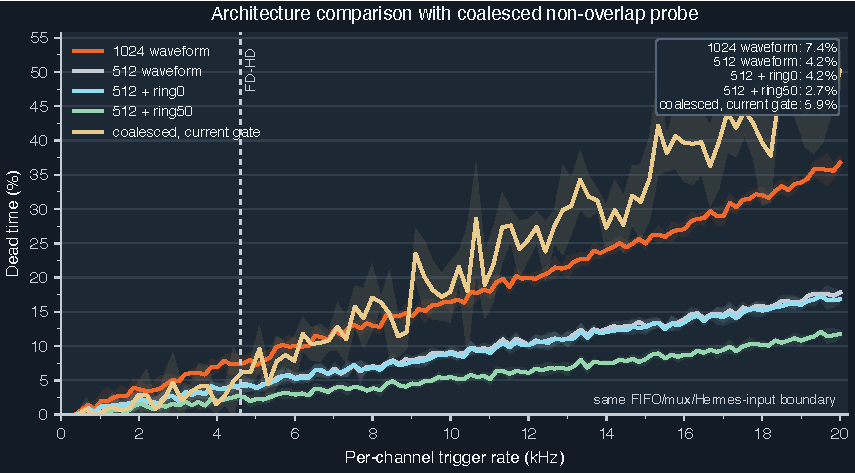
\includegraphics[width=\linewidth,height=0.43\textheight,keepaspectratio]{../daphne_deadtime_apr2026/figures/deadtime_arch_fiveway_dunenoir.pdf}
    \column{0.28\linewidth}
      \eyebrow{Reviewer reading}
      \vspace{1mm}
      {\scriptsize
      512 windows are the first robust improvement.\par
      \vspace{1.5mm}
      Ring50 is the best fixed-record curve.\par
      \vspace{1.5mm}
      Coalesced only becomes excellent after the output gate changes.\par
      \vspace{1.5mm}
      {\color{noirmuted}More lanes are secondary to the window admission contract.}\par}
  \end{columns}
\end{frame}

\begin{frame}{Coalesced Transport: Not Yet A Production Claim}
  \centering
  \resizebox{0.96\linewidth}{!}{%
  \begin{tikzpicture}
    \node[font=\scriptsize,text=noirmuted,anchor=east] at (-0.3,1.1) {old fixed windows};
    \draw[noirline,line width=1pt] (0,1.1) -- (10.8,1.1);
    \fill[noircyan!35] (0.8,0.78) rectangle (3.5,1.42);
    \fill[noircyan!35] (2.7,0.78) rectangle (5.4,1.42);
    \fill[noircyan!35] (4.9,0.78) rectangle (7.6,1.42);
    \node[font=\tiny,text=noirtext] at (2.1,1.65) {duplicate payload can be allowed};
    \node[font=\scriptsize,text=noirmuted,anchor=east] at (-0.3,-0.1) {coalesced interval};
    \draw[noirline,line width=1pt] (0,-0.1) -- (10.8,-0.1);
    \fill[okgreen!45] (0.8,-0.42) rectangle (7.6,0.22);
    \node[font=\tiny,text=noirtext] at (4.2,0.45) {one non-overlapping coverage interval};
    \node[wideblock,text width=2.9cm] (a) at (1.7,-1.7) {Good idea\\merge overlapping windows};
    \node[wideblock,text width=2.9cm] (b) at (5.4,-1.7) {Bad inherited contract\\output gate still counts old frames};
    \node[wideblock,text width=2.9cm,fill=noirpanel] (c) at (9.1,-1.7) {Needed fix\\interval-aware release and backpressure};
    \draw[arrow] (a) -- (b);
    \draw[warrow] (b) -- (c);
  \end{tikzpicture}}
  \vspace{2mm}
  {\color{noirmuted}\footnotesize Coalescing removes duplicate waveform transport, but it only reduces dead time after the downstream frame/queue contract stops behaving like every accepted trigger must reserve a full independent fixed record.\par}
\end{frame}

\begin{frame}{K26 Resources: Does The Design Have Margin?}
  \begin{columns}[T,onlytextwidth]
    \column{0.49\linewidth}
      \eyebrow{Known build references}
      \vspace{1mm}
      \scriptsize
      \begin{itemize}
        \item \texttt{a389fcd}: routed clean baseline.
        \item \texttt{27a4ca9}: ring2k routed clean, but BRAM tight.
        \item grouped Hermes draft: placement failed on BRAM.
        \item xcorr DSP reduction: candidate to trade DSP for CLB/carry logic.
      \end{itemize}
    \column{0.47\linewidth}
      \eyebrow{Resource bars}
      \vspace{1mm}
      \scriptsize
      \textbf{Baseline \texttt{a389fcd}}\\
      \utilbar{CLB LUT}{72.2}{84.5k / 117.1k}{okgreen}\\
      \utilbar{BRAM}{68.8}{99 / 144}{okgreen}\\
      \utilbar{DSP}{99.4}{1240 / 1248}{riskred}\\[1.5mm]
      \textbf{Ring2k \texttt{27a4ca9}}\\
      \utilbar{CLB LUT}{90.0}{105.4k / 117.1k}{warnyellow}\\
      \utilbar{BRAM}{96.5}{139 / 144}{riskred}\\
      \utilbar{DSP}{96.2}{1200 / 1248}{riskred}\\[1.5mm]
      \textbf{Grouped draft}\\
      \utilbar{BRAM}{105.6}{152 / 144}{riskred}
  \end{columns}
  \vspace{2mm}
  {\color{noirmuted}\footnotesize Dead-time mitigation competes directly with BRAM/LUT/DSP margin. The next architecture must remove replication deliberately, not add another layer of FIFOs.\par}
\end{frame}

\begin{frame}{Transport: Production Versus Study}
  \centering
  \resizebox{0.97\linewidth}{!}{%
  \begin{tikzpicture}
    \node[font=\small\bfseries,text=noircyan] at (0,2.5) {Current production-compatible shape};
    \node[block,text width=2.2cm] (c1) at (0,1.5) {40 logical\\channel builders};
    \node[block,text width=2.2cm] (c2) at (3,1.5) {40-slot\\mux};
    \node[block,text width=2.2cm] (c3) at (6,1.5) {2 Hermes\\lanes};
    \draw[arrow] (c1) -- (c2);
    \draw[arrow] (c2) -- (c3);
    \node[font=\small\bfseries,text=noircyan] at (0,-0.1) {Architecture study target};
    \node[block,text width=2.2cm,fill=noirpanel] (n1) at (0,-1.1) {40 local rings\\+ compact queues};
    \node[block,text width=2.2cm,fill=noirpanel] (n2) at (3,-1.1) {late grouped\\packet assembly};
    \node[block,text width=2.2cm,fill=noirpanel] (n3) at (6,-1.1) {direct grouped\\Hermes handoff};
    \draw[arrow] (n1) -- (n2);
    \draw[arrow] (n2) -- (n3);
    \node[riskblock,text width=3.2cm] at (10,1.5) {Good for compatibility\\but expensive replication};
    \node[riskblock,text width=3.2cm] at (10,-1.1) {Better architecture\\but must prove BRAM and dead time};
  \end{tikzpicture}}
  \vspace{2mm}
  {\color{noirmuted}\footnotesize Design principle: do not jump to 5 AFE producers just because it is cheaper. It risks cross-channel blocking. Prefer local channel storage with late grouped assembly sized by simulation and BRAM budget.\par}
\end{frame}

\sectioncard{Reviewable Claims}{Every production claim should map to evidence, an owner, and a fallback. That is the PRR package.}

\begin{frame}{Which Claims Are Ready For Review?}
  \begin{columns}[T,onlytextwidth]
    \column{0.49\linewidth}
      \panelbox{Production reference: \oktag}{The routed firmware baseline and overlay packaging path exist. Keep this as the comparison point for any mitigation branch.}
      \vspace{3mm}
      \panelbox[panel alt]{DAQ descriptor chain: \worktag}{Format bindings, raw-data extraction, monitoring, and waffles integration exist on active branches. The missing PRR item is a reviewed release path with tests.}
    \column{0.49\linewidth}
      \panelbox[panel alt]{Mezzanine noise filters: \unknowntag}{The mitigation is credible, but production readiness needs before/after spectra, a schematic/BOM delta, and an acceptance test.}
      \vspace{3mm}
      \panelbox{Dead time and PDS trigger: \risktag}{Simulations clarify the choices, but the production architecture and trigger primitive owner group are still open risks.}
  \end{columns}
  \vspace{4mm}
  {\color{noirmuted}\footnotesize Backups keep the detailed source map; the main deck stays decision-oriented.\par}
\end{frame}

\begin{frame}{Evidence Packet The Panel Should Expect}
  \centering
  \resizebox{0.97\linewidth}{!}{%
  \begin{tikzpicture}
    \node[reviewblock,text width=3.2cm] (req) at (0,0) {\textbf{Requirements}\\rate, dead time, noise, links, controls};
    \node[reviewblock,text width=3.2cm] (icd) at (4.05,0) {\textbf{Interfaces}\\mezzanine, AFE, PL, DAQ, trigger primitives};
    \node[reviewblock,text width=3.2cm] (ver) at (8.1,0) {\textbf{Verification}\\lab tests, sim, routed builds, DAQ playback};
    \node[reviewblock,text width=3.2cm] (prod) at (12.15,0) {\textbf{Production}\\BOM, assembly, QA/QC, acceptance};
    \draw[arrow] (req) -- (icd);
    \draw[arrow] (icd) -- (ver);
    \draw[arrow] (ver) -- (prod);
    \node[reviewblock,text width=3.2cm,below=1.0cm of req] (risk) {\textbf{Risk register}\\dead time, noise, resources, ownership};
    \node[reviewblock,text width=3.2cm,below=1.0cm of icd] (owner) {\textbf{Owners}\\hardware, firmware, DAQ, PDS trigger};
    \node[reviewblock,text width=3.2cm,below=1.0cm of ver] (fall) {\textbf{Fallbacks}\\fixed 512/ring50, no coalesced, reduced feature set};
    \node[reviewblock,text width=3.2cm,below=1.0cm of prod] (sched) {\textbf{Schedule}\\decision dates, dry run, PRR closure actions};
    \draw[greyarrow] (risk) -- (owner);
    \draw[greyarrow] (owner) -- (fall);
    \draw[greyarrow] (fall) -- (sched);
  \end{tikzpicture}}
  \vspace{2mm}
  {\color{noirmuted}\footnotesize The PRR deck should point to one controlled evidence matrix, not ask reviewers to infer status from many branches.\par}
\end{frame}

\begin{frame}{PDS Trigger Ownership: The Risk To Challenge}
  \centering
  \resizebox{0.88\linewidth}{!}{%
  \begin{tikzpicture}
    \node[wideblock,fill=noirpanel] (pd) at (0,0) {Peak descriptor\\firmware product};
    \node[wideblock] (tp) at (4.0,0) {Trigger primitive\\DAQ/PDS contract};
    \node[wideblock] (alg) at (8.0,0) {PDS trigger algorithm\\physics responsibility};
    \node[wideblock] (ops) at (12.0,0) {Operations\\monitoring and alarms};
    \draw[arrow] (pd) -- (tp);
    \draw[warrow] (tp) -- (alg);
    \draw[arrow] (alg) -- (ops);
    \node[riskblock,below=0.9cm of tp,text width=3.2cm] {Current weak seam: who owns primitive definition and validation?};
  \end{tikzpicture}}
  \vspace{7mm}
  \begin{columns}[T,onlytextwidth]
    \column{0.48\linewidth}
      \panelbox{What we have}{Firmware can produce peak descriptors, and DAQ can expose them to monitoring and analysis.}
    \column{0.48\linewidth}
      \panelbox[panel alt]{What is still missing}{A named owner group and acceptance tests for descriptor-to-trigger-primitive behavior.}
  \end{columns}
\end{frame}

\begin{frame}{Is This Ready To Become The PRR Package?}
  \begin{columns}[T,onlytextwidth]
    \column{0.48\linewidth}
      \panelbox{Yes, as a draft}{The existing presentations, firmware docs, dead-time simulations, DAQ branches, and hardware schematics are enough to draft the PRR story and identify the main open risks.}
      \vspace{3mm}
      \panelbox[panel alt]{No, not as the final review package}{It is not clean enough yet for DOE reviewers because the evidence is spread across repos and branches, and some fronts are status notes rather than acceptance criteria.}
    \column{0.48\linewidth}
      \eyebrow{Reviewer-facing cleanup}
      \begin{itemize}
        \item One readiness matrix with owner, evidence, status, and next action.
        \item One interface-control view from AFE to DAQ trigger primitives.
        \item One dead-time requirement and one accepted operating model.
        \item One hardware noise validation plan for the mezzanine filters.
        \item One DAQ release path for descriptor extraction and monitoring.
      \end{itemize}
  \end{columns}
\end{frame}

\begin{frame}{Narrative The Panel Can Follow}
  \centering
  \resizebox{0.96\linewidth}{!}{%
  \begin{tikzpicture}
    \node[reviewblock,text width=3.0cm] (one) at (0,0) {\textbf{1. Role}\\DAPHNE is the common warm PDS readout interface.};
    \node[reviewblock,text width=3.0cm] (two) at (3.95,0) {\textbf{2. Hardware}\\Mezzanine flexibility solves input technology differences; new filters address noise.};
    \node[reviewblock,text width=3.0cm] (three) at (7.9,0) {\textbf{3. Firmware}\\Matched filter and descriptors are useful, but resource/dead-time tradeoffs are real.};
    \node[reviewblock,text width=3.0cm] (four) at (11.85,0) {\textbf{4. DAQ}\\Descriptor extraction chain is being integrated into standard packages.};
    \node[reviewblock,text width=3.0cm] (five) at (15.8,0) {\textbf{5. Decision}\\Freeze what is production, track what is mitigation, assign trigger ownership.};
    \draw[arrow] (one) -- (two);
    \draw[arrow] (two) -- (three);
    \draw[arrow] (three) -- (four);
    \draw[arrow] (four) -- (five);
  \end{tikzpicture}}
  \vspace{6mm}
  \begin{beamercolorbox}[wd=0.92\linewidth,sep=7pt,rounded=true]{panel}
    \centering
    \textbf{Main message for reviewers:} DAPHNE is close enough for a serious PRR package, if dead time and trigger primitives are presented as controlled production risks with owners and fallbacks.
  \end{beamercolorbox}
\end{frame}

\begin{frame}{Closure Plan Before Review}
  \centering
  \resizebox{0.98\linewidth}{!}{%
  \begin{tikzpicture}
    \node[wideblock,text width=3.2cm,fill=noirpanel] (a) at (0,0) {Freeze PRR scope\\build evidence matrix};
    \node[wideblock,text width=3.2cm] (b) at (4.3,0) {Close descriptor DAQ tests\\prepare monitoring demo};
    \node[wideblock,text width=3.2cm] (c) at (8.6,0) {Package mezzanine noise evidence\\define dead-time acceptance model};
    \node[wideblock,text width=3.2cm] (d) at (12.9,0) {Dry run\\reviewer-readable deck\\risk and fallback decisions};
    \draw[arrow] (a) -- (b);
    \draw[arrow] (b) -- (c);
    \draw[arrow] (c) -- (d);
  \end{tikzpicture}}
  \vspace{5mm}
  \begin{columns}[T,onlytextwidth]
    \column{0.33\linewidth}
      \statcard{Surface risk early}{Dead-time and ownership are better shown as controlled risks than discovered by reviewers.}
    \column{0.33\linewidth}
      \statcard{Credible fallback}{Fixed 512/ring50 is the compatibility fallback while coalesced transport matures.}
    \column{0.33\linewidth}
      \statcard{Make it testable}{Every claim should point to one plot, report, run, or package test.}
  \end{columns}
\end{frame}

\appendix
\sectioncard{Backup}{Sources, resource glossary, and detailed references for technical questions.}

\begin{frame}{Backup: Source Map}
  \scriptsize
  \begin{tabularx}{\linewidth}{@{}p{3.2cm}p{3.7cm}X@{}}
    \toprule
    Front & Local source & What it contributes \\
    \midrule
    Firmware build and resources & \texttt{daphne-firmware/docs} & routed baseline, packaging boundary, architecture drafts, K26 constraints \\
    Dead-time simulations & \texttt{daphne\_mezz\_xc\_sim/docs} & C++ and RTL dead-time studies, ring/coalesced comparisons \\
    Legacy mezzanine firmware & \texttt{Daphne\_MEZZ} & original DAPHNE V3/MEZZ PL and Vivado script reference \\
    Data format & \texttt{fddetdataformats} & DAPHNE Ethernet frame and peak descriptor bindings \\
    Data extraction & \texttt{rawdatautils} & numpy arrays for waveform and peak descriptor fields \\
    Monitoring / control & \texttt{daphnemodules} & DAQ control and online monitoring integration \\
    Analysis & \texttt{waffles} & waveform/descriptor attachment for analysis workflows \\
    \bottomrule
  \end{tabularx}
\end{frame}

\begin{frame}{Backup: Resource Glossary}
  \begin{columns}[T,onlytextwidth]
    \column{0.32\linewidth}
      \panelbox{CLB / LUT}{General FPGA logic. Used by state machines, muxes, counters, control logic, adders, and shift/add filter implementations.}
    \column{0.32\linewidth}
      \panelbox{BRAM / URAM}{On-chip memories. Used by waveform rings, FIFOs, spy buffers, queues, and large buffers.}
    \column{0.32\linewidth}
      \panelbox{DSP48E}{Dedicated arithmetic slices. Used by multiply/filter-heavy paths; the matched filter used to consume most of them.}
  \end{columns}
  \vspace{2mm}
  {\color{noirmuted}\footnotesize If one resource class is above roughly 90--95\%, small design changes can break placement, timing, or routing even when the HDL is functionally correct.\par}
\end{frame}

\begin{frame}{Backup: Dead-Time Takeaway}
  \begin{columns}[T,onlytextwidth]
    \column{0.50\linewidth}
      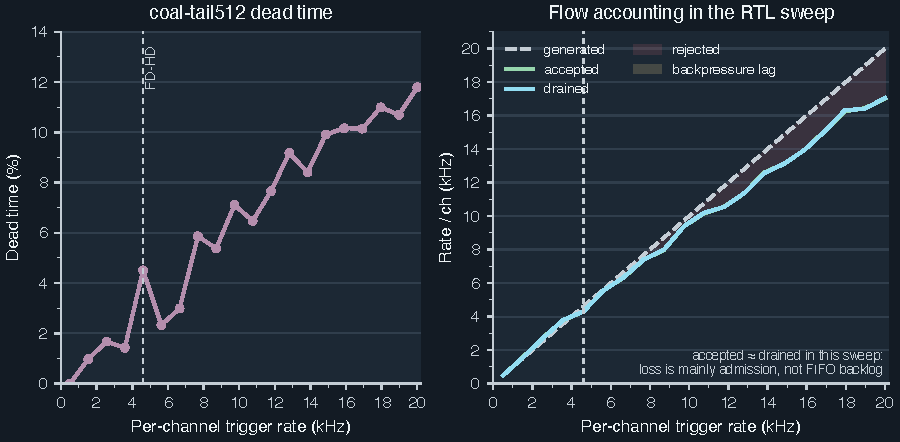
\includegraphics[width=\linewidth,height=0.66\textheight,keepaspectratio]{../daphne_deadtime_apr2026/figures/deadtime_coal_tail512_compact.pdf}
    \column{0.46\linewidth}
      \eyebrow{Plain-English summary}
      \begin{itemize}
        \item 1024-sample records waste too much acceptance.
        \item 512-sample records are a safe first cut.
        \item Ring50 improves dead time while keeping the fixed-record contract.
        \item Coalesced transport is the long-term clean idea, but only if the output queue semantics change too.
      \end{itemize}
  \end{columns}
\end{frame}

\end{document}
